\documentclass[11pt,twoside]{report}
\usepackage{preamble}
\graphicspath{{../img/ch1/}}
\setcounter{chapter}{0}


\begin{document}


\chapter{Introduction}

This thesis will discuss the \emph{collective behaviour} of \emph{zebrafish}. And we will start the thesis by describing the individual terms of our topic.

\section{Collective Behaviour}

When objects were densely-packed together, interesting phenomena  appear. And we could call these phenomena as the \emph{collective behaviour} of these things. The collective behaviour is interesting because ``more is different'' \cite{anderson1972}. In other words, the behaviour of a large group can not be predicted, even if we know precisely the fundamental laws for the individuals.

An example to illustrate the complexity of collective behaviour, is a collection of randomly packed balls. When we randomly pack a lot of plastic balls together, they packed together like those in Fig.~\ref{fig:random-pack}. These plastic balls, often modelled as \emph{hard spheres}, have a simple property that two spheres can not be too close so that they overlap.
Surprisingly, the accurate prediction of the density (expressed for example as the volume fraction) of the randomly packed hard spheres is still unachieved\marginfootnote{
The latest progress about this problem was made by \citeauthor{zaccone2022} \cite{zaccone2022}. But the proposed solution received many criticisms \cite{blumenfeld2022, charbonneau2022, chen2022}.
} \cite{kamien2007, zaccone2022}.
In addition, the well packed hard spheres form a collection of clusters with different geometrical features. In Fig.~\ref{fig:random-pack} two different clusters were highlighted. The prediction of the geometrical features is still a challenging problem \cite{malins2013, robinson2019}.

The collective behaviour of objects with varying lenght-scales were studied, from atoms, to colloids, animals, as well as human beings \cite{walker1990, lekkerkerker1992, becco2006, henderson1971, silverberg2013}. The interesting feature of their collective behaviour is the transformation from one phase to another under different conditions \cite{sethna2006}. For instance, the water could change between the fluid phase and crystal phase under different temperatures. These behaviours are often noted as \emph{phase behaviour}, and summarised by \emph{phase diagrams}. The phase diagrams of systems in equilibrium have been systematically studied. However, the equivalent in non-equilibrium systems were less studied, and they will be introduced in chapter~\ref{chapter:collective_behaviour}.

\marginpar{
\centering
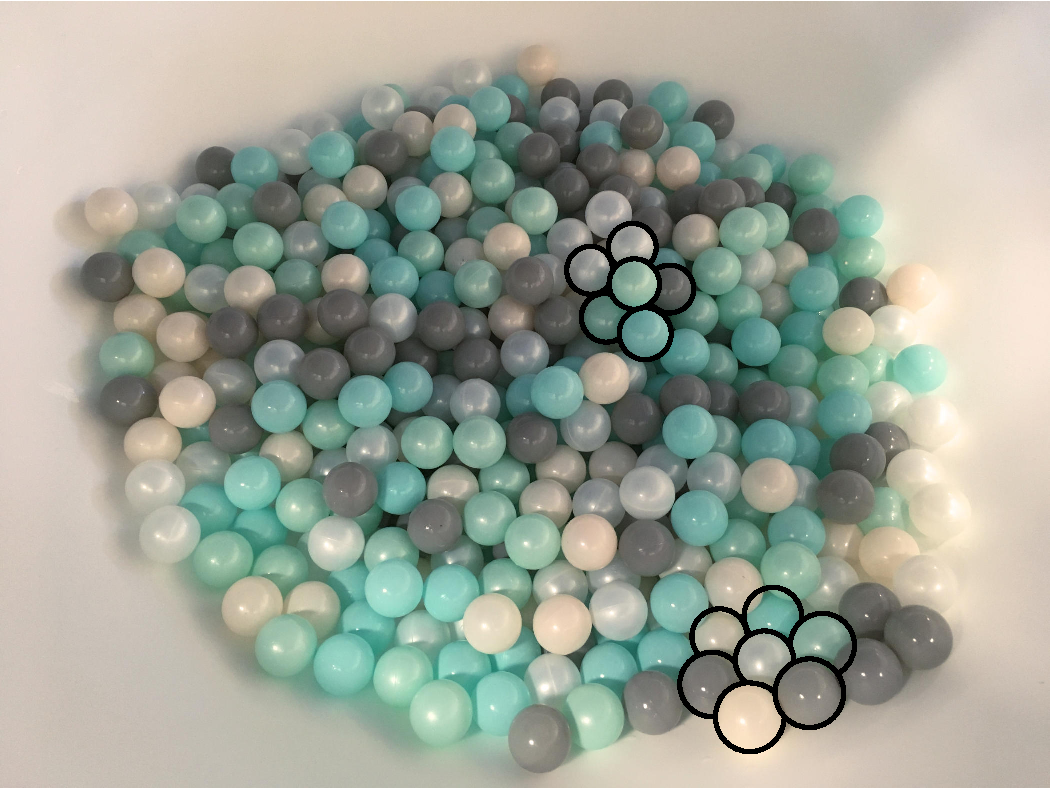
\includegraphics[width=\marginparwidth]{random-pack}
\captionof{figure}[Randomly packed plastic balls.]{
  A photo of randomly packed plastic balls. The photo was taken by the author.
}
\label{fig:random-pack}
}


\section{Zebrafish}

Zebrafish (\emph{Danio rerio}) is a small fish living mainly in  India and Bangladesh, as well as in areas of Pakistan, Nepal, and Myanmar \cite{neff2020}. These fish are social animals that form small groups in the size of tens in still water \cite{suriyampola2016}. In rivers with faster flow, the group size could be thousands \cite{shelton2020}. The photo of a typical adult zebrafish is shown in Fig.~\ref{fig:fish}, with the characteristic stripes of this species. Placing a group of these fish together, they will interact with each other, and often form a coherent group. These behaviours are what we will be studying through out this thesis.


\marginpar{
\centering
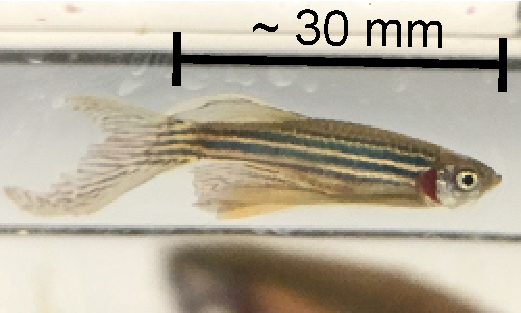
\includegraphics[width=\marginparwidth]{zebrafish}
\captionof{figure}[The photo of a zebrafish]{
	The photo of an adult zebrafish. The photo was taken by the author.
}
\label{fig:fish}
}

Zebrafish receive attention from the scientific community, because they present a good animal model for different human diseases. Being a vertebrate, the genome of zebrafish is similar to that of human beings \cite{howe2013}. In addition, the embryo of zebrafish, as well as the zebrafish larva are transparent \cite{kimmel1995}, making microscopic observation of cellular behaviour very easy. With the help of zebrafish, we could study common diseases such as the osteoarthritis \cite{lawrence2018, kague2021}, autism \cite{kim2017}, and cancer \cite{lopez-cuevas2021}. The appeal of zebrafish as an animal model makes them being widely used in different institutions\cite{spence2007}. Practically, the zebrafish in the laboratory were kept in a standard condition for many generations \cite{westerfield2000}. These fish are less likely to suffer from common diseases and parasites, comparing with wild captivated fish \cite{spence2007}. These fish are good for behavioural experiment as their living condition are controlled, which makes repeating experiments easy. In this thesis, all the zebrafish were bred at the fish facility of the University of Bristol.

There are multiple reasons to study the collective behaviour of the zebrafish. The first reason is technical. The fish naturally swim in the river, where they can change their depth every now and then. Observing the fish swimming in a three dimensional (3D) space requires advanced tracking system. The design and construction of such 3D underwater tracking system is a technical challenge. And it is meaningful to solve this challenge. In addition, understanding the behaviour of zebrafish could help us differentiate the states of the fish. And we will have predictive power about the fish behaviour, if we could construct a phase diagram of the fish. Finally, we may study the behavioural difference of the mutant zebrafish, to understand the consequences of genetic modifications.


\section{Thesis Structure}


In the next chapter the ideas of active matter and the collective behaviour of animals will be discussed.
We will draw the similarity between a group of animal and a group of synthetic particles under constant energy input. 
Typically, we will stress the complex patterns formed by the animals. The statistical analysis of these patterns will be discussed, as well as some mathematical models that explained the behaviour.

The following two chapters, chapter~\ref{chapter:fish_2d} and \ref{chapter:fish_3d}, will address the technical challenges for the construction of a 3D fish tracking system. Firstly, the method to record the 2D movements of the zebrafish will be discussed in chapter \ref{chapter:fish_2d}. The important element in chapter~\ref{chapter:fish_2d} is the image processing methods, which enables us to extract features from the images. The density distribution of the fish in a quasi-2D environment will also be discussed in chapter~\ref{chapter:fish_2d}. 
Then we will move to chapter~\ref{chapter:fish_3d}, which discussed the construction of a 3D tracking system. 
This chapter will mainly feature different algorithms to calculate the 3D locations of the fish, following the ideas  of multiple view geometry. The experimental results of 3D tracking will also be discussed in chapter \ref{chapter:fish_3d}.


The tracking system will first produce the coordinates of the fish, which provides the information about the structure of the fish group. To study the dynamics of the fish, the coordinates needs to be linked into trajectories. The linking method will be introduced in chapter~\ref{chapter:fish_analysis}. From the trajectories, we can study the structure and the dynamics of the fish with analytical methods developed in the active-matter community. The analysis includes the calculation of different quantities that capture the essence of the fish behaviour, as well as the calculation of the \emph{correlations} of different quantities. These analytical methods will be introduced, and applied to the experimental data. As a result, an important behavioural feature of the fish will be revealed in the end of chapter~\ref{chapter:fish_analysis}.


To further understand the fish behaviour, typically the analytical results, we will try to construct models that reproduced the behaviour. We will model the fish as identical agents following certain rules. We will make the model behave like the real fish, by adjusting the model parameters to match the analytical results. The fitted model will then serve as explanations for the observed results. Specifically, we will try to understand the density distribution of the fish, as well as the dynamics of the fish with different models.


Afterwards, we will move to a more biological topic and discuss the behaviour of zebrafish after genetic modification. In chapter \ref{chapter:fish_mutation}, the collective behaviour of the mutant fish will be reported and compared against the normal, wildtype zebrafish.
%The insight into the mutation fish is only available through the behavioural experiments, as t
The mutant fish have a longer orientational relaxation time compared with the wildtype fish.
The change in the single-fish property will affect the collective behaviour of the fish, making a group of mutant fish exhibiting more ordered movement, which can be explained by an active matter model from chapter~\ref{chapter:fish_model}.


Finally, we close the thesis with a conclusion that summarised all experimental observations, analytical results, as well as the models, and discussed possible future tasks to further improve our understand of the zebrafish behaviour.

\end{document}